\item O bloco $A$ de \SI{20}{\kilogram} é rebocado para cima na rampa do carrinho de \SI{40}{\kilogram} usando-se o motor $M$ montado ao lado do carrinho. Se o motor enrola o cabo a uma velocidade constante de \SI{5}{\meter/\second}, medida
relativamente ao carrinho, determine a distância que o carrinho percorrerá quando o bloco tiver viajado uma distância $s=\SI{2}{\meter}$, rampa acima. Tanto o bloco quanto o carrinho estão em repouso quando $s=0$. O coeficiente de atrito
cinético entre o bloco e a rampa é $\mu_{k}=0.2$. Despreze a resistência
ao rolamento.


\vspace{-.7cm}
\begin{flushright}
	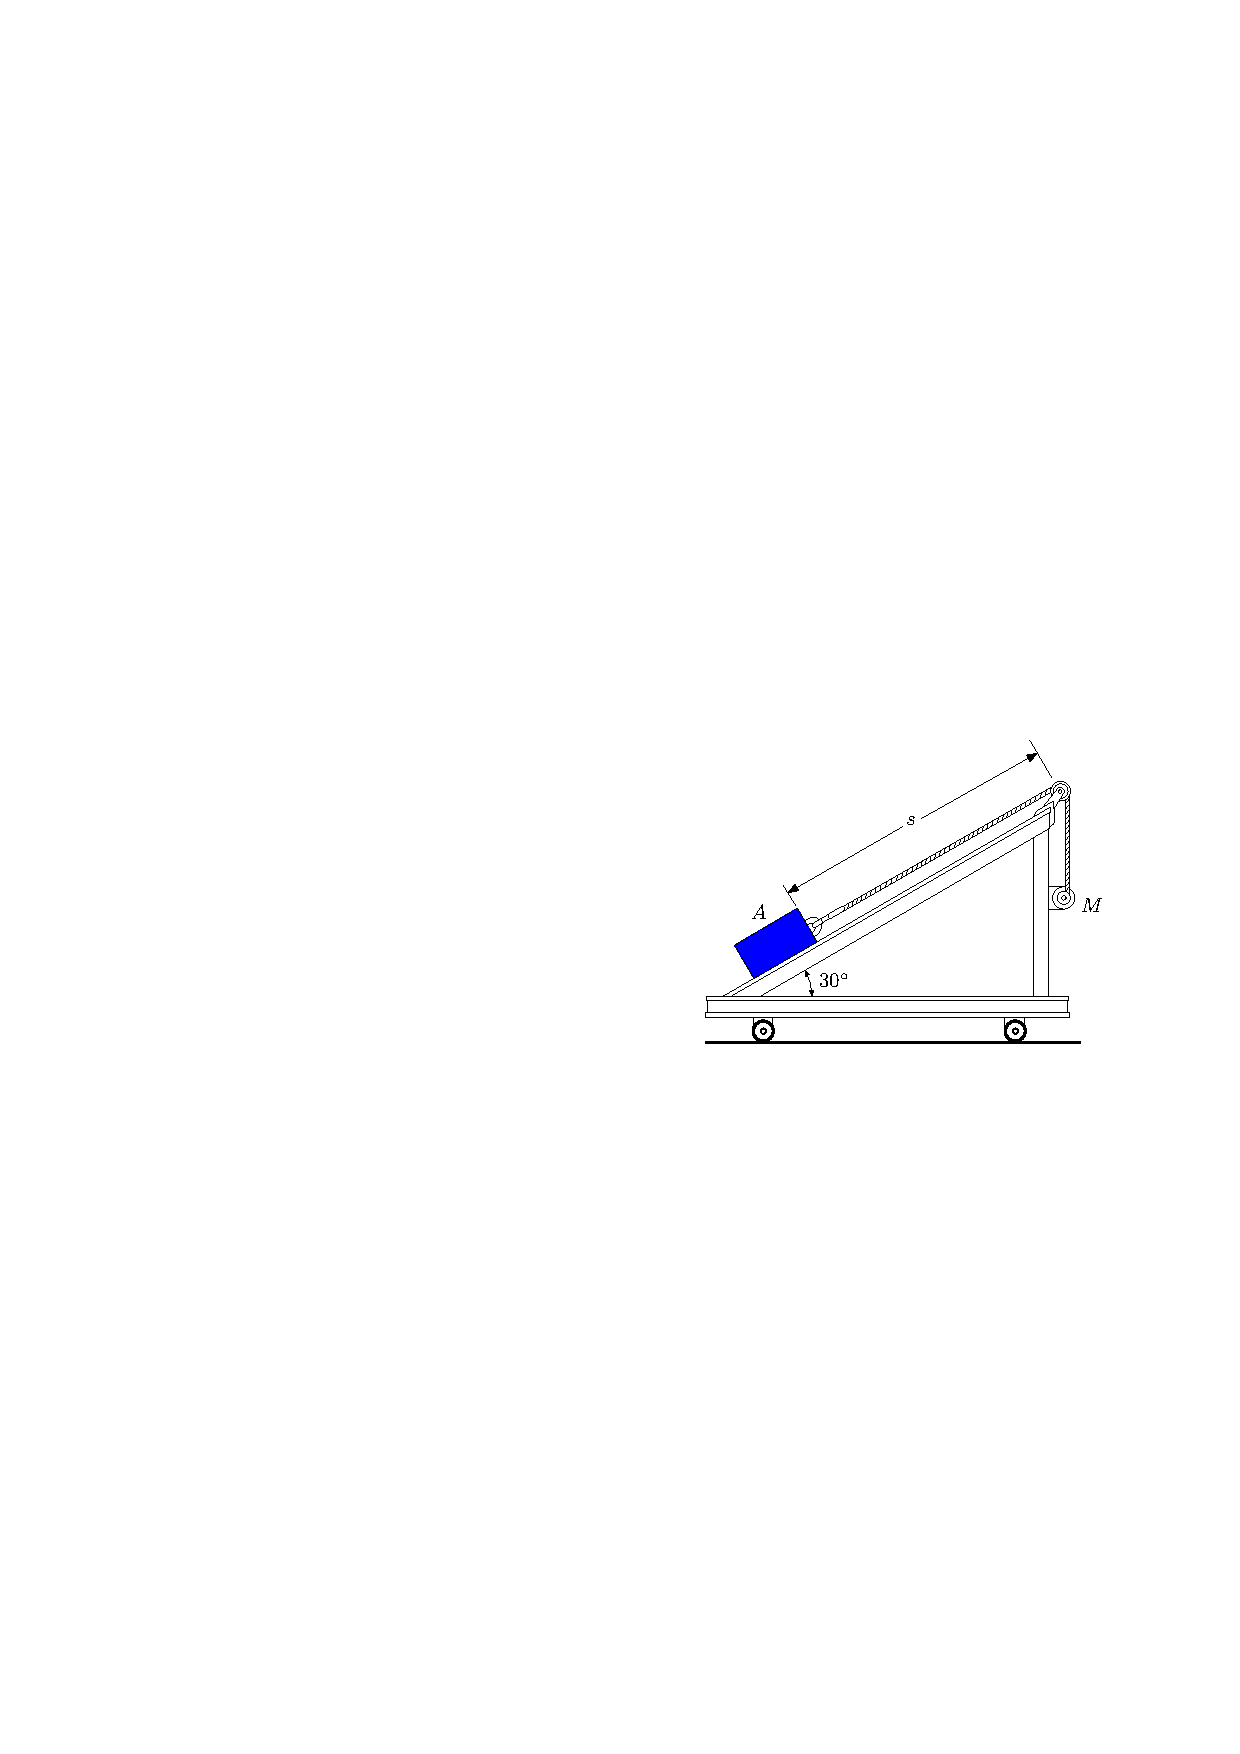
\includegraphics[scale=1.3]{images/draw_4}
\end{flushright}